\documentclass[11pt]{article} % use larger type; default would be 10pt
\usepackage[utf8]{inputenc} % set input encoding (not needed with XeLaTeX)

\usepackage{amsfonts,amsthm,amsmath,amssymb}
\usepackage{array}
\usepackage{epsfig}
\usepackage{fullpage}
\usepackage{enumerate}
\usepackage[hidelinks]{hyperref}
\usepackage{color}
\usepackage{algorithm}
\usepackage{comment}\usepackage{amsfonts,amsthm,amsmath,amssymb}
\usepackage{array}
\usepackage{epsfig}
\usepackage{fullpage}
\usepackage{enumerate}
\usepackage[hidelinks]{hyperref}
\usepackage{color}
\usepackage{algorithm}
\usepackage{comment}
\usepackage{cryptocode}
\usepackage{graphicx}
\usepackage{url}
\usepackage{subcaption}
\usepackage{mathpartir}

\usepackage[hyperpageref]{backref} %% puts links to the page numbers where a bib entry is cited after the bib entry---particularly useful for getting back to where you started after clicking on a citation

\usepackage[numbers]{natbib}  % Enables numbered citations
\bibliographystyle{plainnat}  % A numeric style compatible with natbib
\hypersetup{
    colorlinks=true,
    linkcolor=purple,
    filecolor=purple,      
    urlcolor=purple,
    citecolor=purple
    }


\usepackage{mathtools}  
\usepackage{diffcoeff}  

\renewcommand{\vec}{\mathbf}


\newcounter{algo}
\newenvironment{algo}[1]
  {\refstepcounter{algo}
    \medskip
    \noindent\rule{\columnwidth}{1pt} \nopagebreak
    {\bf Algorithm #1} 

    \nopagebreak 
    \noindent\rule{\columnwidth}{0.4pt}

    \small\noindent
  }
  {\noindent\rule{\columnwidth}{1pt}
  \medskip
  }

\newcommand{\EC}{\textbf{(EC)} }

\newcommand{\Gen}{\mathsf{Gen}}
\newcommand{\Enc}{\mathsf{Enc}}
\newcommand{\Dec}{\mathsf{Dec}}
\newcommand{\Samp}{\mathsf{Samp}}
\newcommand{\Comp}{\mathsf{Comp}}

\newcommand{\MAC}{\mathsf{MAC}}
\newcommand{\Sign}{\mathsf{Sign}}
\newcommand{\Ver}{\mathsf{Ver}}

\newcommand{\negl}{\mathsf{negl}}
\newcommand{\bad}{\mathsf{BAD}}
\newcommand{\uu}{\mathcal{U}}

\newcommand{\adversary}{\mathcal{A}}
\newcommand{\bb}{\mathcal{B}}
\newcommand{\mm}{\mathcal{M}}

\newcommand{\M}{\mathcal{M}}
\newcommand{\C}{\mathcal{C}}
\newcommand{\K}{\mathcal{K}}
\def\zo{\{0,1\}}
%\newcommand{\from}{\leftarrow}
\newcommand{\eps}{\varepsilon}
\renewcommand{\epsilon}{\varepsilon}
\usepackage{enumitem}

\newcommand{\nnote}[1]{{\color{blue} \footnotesize(Noah: #1)}}
% \newcommand{\nnote}[1]{}
\newcommand{\A}{\mathcal{A}}

\newcommand\extlines[1]{%
	\setcounter{index}{0}%
	\whiledo {\value{index}< #1}
	{\addtocounter{index}{1}\extline}
}

%\newcommand\rextlinearrow[2]{$
%  \setbox0\hbox{$\extlines{#2}\rextlineend$}%
%  \tiny$%
%  \!\!\!\!\begin{array}{c}%
%  \mathrm{#1}\\%
%  \usebox0%
%  \end{array}%
%  $\normalsize$\!\!%
%}
%
%\newcommand\lextlinearrow[2]{$
%  \setbox0\hbox{$\lextlineend\extlines{#2}$}%
%  \tiny%
%  $%
%  \!\!\!\!\begin{array}{c}%
%  \mathrm{#1}\\%
%  \usebox0%
%  \end{array}%
%  $\normalsize$\!\!%
%}

\newcommand\lextlinearrow[1]{%
	$\xleftarrow{\mathmakebox[.4\hsize]{\shortstack{$#1$}}}$
}

\newcommand\rextlinearrow[1]{%
	$\xrightarrow{\mathmakebox[.4\hsize]{\shortstack{$#1$}}}$
}

\newlength{\protocollength}
\setlength{\protocollength}{0.98\textwidth}


\newcommand{\protocol}[1]{
	\small
	%\begin{center}
	\begin{tabular}{l c l}
	%{\protocollength}{>{\hsize=1\hsize}X >{\hsize=1\hsize}X >{\hsize=1\hsize}X}
% 	\begin{tabu}%to\protocollength{X X[-.8] X}
		%\hline
		{\bfseries Adversary} & & {\bfseries Challenger}\\
		%\multicolumn{1}{c}{\bf Alice}&&
		%$\procedure{}\ \mathrm{Alice}(m)$ & &
		%\multicolumn{1}{c}{\bf Bob}\\
		%$\procedure{}\ \mathrm{Bob}()$\\
		%\hline
		\hline
		%\rule{4 cm}{0pt}&\rule{5 cm}{0pt}&\rule{4 cm}{0pt}\\
		#1
% 	\end{tabu}
	\end{tabular}
	%\end{center}
}
\newcommand{\bobtoalice}[1]{& \lextlinearrow{#1}&\\}
%\newcommand{\notbobtoalice}[1]{& \lextlinearrow{\xcancel{#1}}{26}&\\}
\newcommand{\alicetobob}[1]{& \rextlinearrow{#1}&\\}
%\newcommand{\notalicetobob}[1]{& \rextlinearrow{\xcancel{#1}}{26}&\\}
\newcommand{\boxalicetobob}[1]{& \begin{boxedminipage}{15 em} \rextlinearrow{#1}{26} \end{boxedminipage}&\\}
\newcommand{\bobcompute}[1]{&& #1\\}
\newcommand{\alicecompute}[1]{#1 &&\\}
\newcommand{\cominput}[1]{\texttt{INPUT: }$#1$}
\newcommand{\comif}{\texttt{IF\ }}
\newcommand{\comfor}{\texttt{FOR\ }}
\newcommand{\comand}{\texttt{AND\ }}
\newcommand{\comor}{\texttt{OR\ }}
\newcommand{\comelse}{\texttt{ELSE}}
\newcommand{\comreturn}{\texttt{RETURN\ }}
\newcommand{\comoutput}{\texttt{OUTPUT\ }}

\NewEnviron{solution}[1][\vspace{0pt}]{
    
    {\vspace{10pt} \textcolor{blue}{
    \BODY $\hfill\blacksquare$
    \vspace{10pt}}}
    {#1}  
}



%%% END Article customizations

%%% The "real" document content comes below...

\title{Prefix-Tuning}
%\date{} % Activate to display a given date or no date (if empty),
         % otherwise the current date is printed 
\author{Mac Turner, Michael Ngo, Eric Hu, Neeraj Parihar}

\begin{document}
\maketitle

\section{Introduction}
Finetuning LLMs for specific tasks requires training a new set of weights for every task, which is expressive but expensive. On the other hand, prompt engineering does not require any training, which is cheap but limiting. \textit{Prefix-Tuning: Optimizing Continuous Prompts for Generation} by Xiang Lisa Li and Percy Liang~\cite{li-liang-2021-prefix} introduces a method of fine-tuning that is combines the efficiency of prompt engineering and the effectiveness of full fine tuning.

The paper shows that prefix tuning GPT-2, BART and T5 on table-to-text generation and text summarization performs better than fine tuning and other parameter efficient fine tuning methods. Additionally, prefix tuning is more parameter efficient and thus faster to train than other fine tuning methods.

\section{Chosen Result}

We chose to reproduce prefix-tuning for GPT-2 Medium on table-to-text generation and compare it against full fine tuning. This is the first two rows and the first column of Table 1 in the original paper, shown in Figure 1. We chose this because it's the first major result of the paper that prefix-tuning is comparable, if not better than fine tuning, and GPT-2 and the E2E table-to-text dataset used were the simplest models and datasets to set up.

\begin{figure}
    \centering
    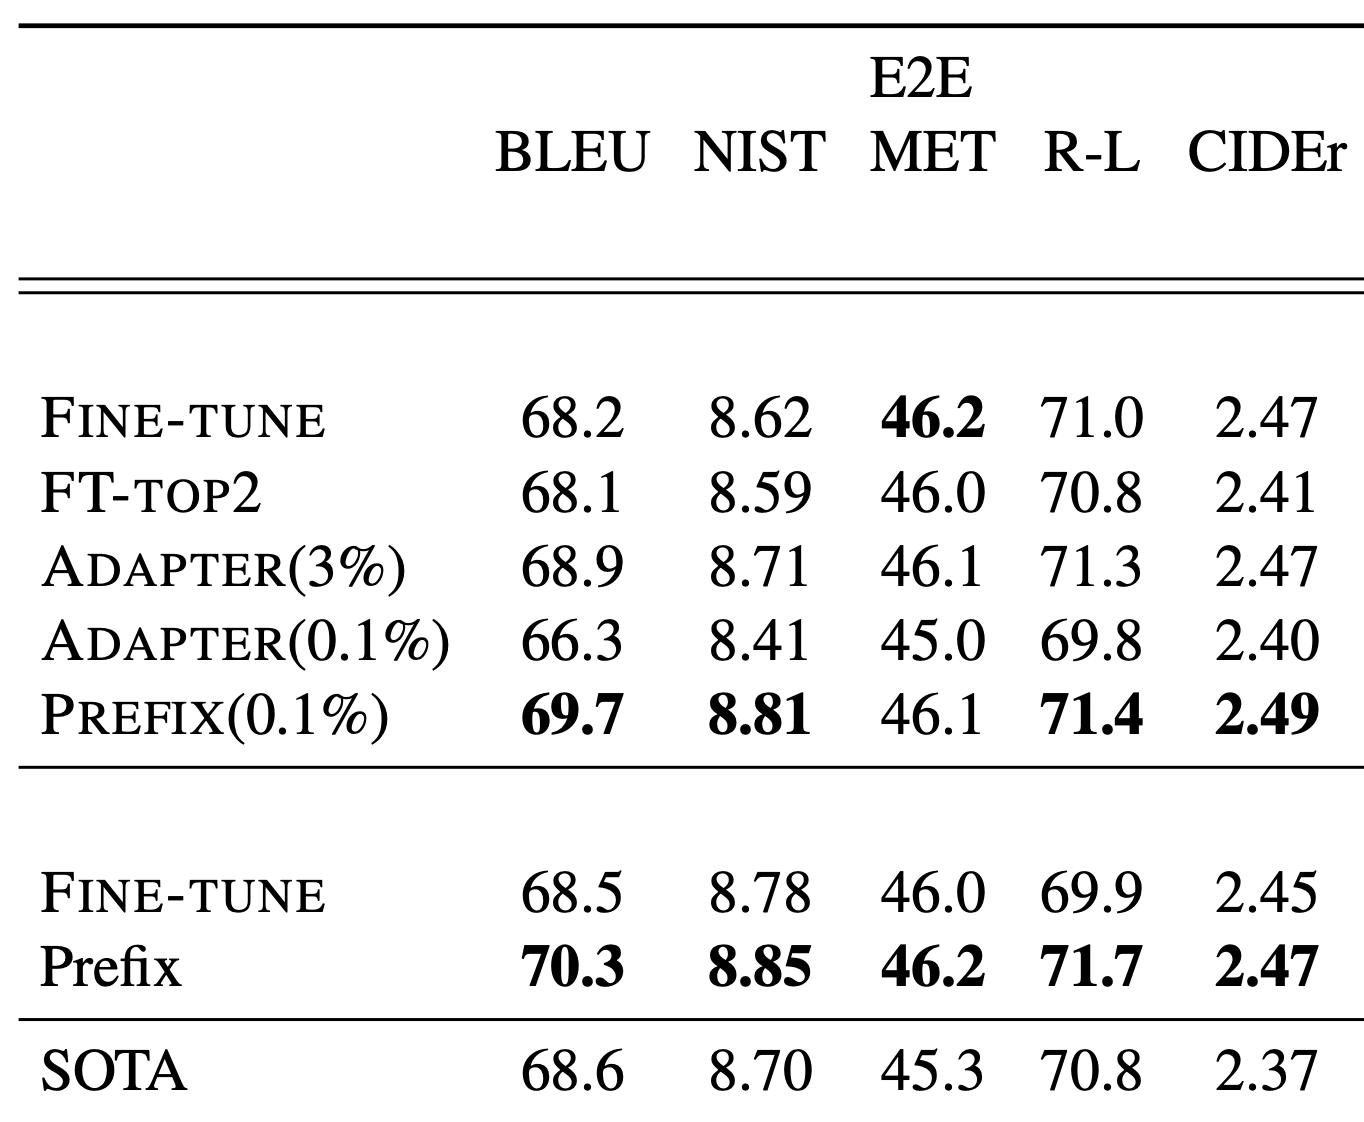
\includegraphics[width=0.5\linewidth]{table1.png}
    \caption{Table 1 from the original paper}
    \label{fig:enter-label}
\end{figure}

\section{Methodology}

\subsection{Prefix-Tuning}
The base model we freeze is GPT-2 Medium. The model is a stack of attention blocks with hidden size $d=768$. For each attention block $i$, we learn the first $L$ keys and values via a network, $\textsf{MLP}_{\theta,i}$ and input matrix $P_{\theta,i}$. $P_{\theta,i}$ is of dimension $L\times d$. The MLP is 2 layers, specifically a linear layer from $d$ to $d_i$ (where $d_i$ is an intermediate size we set to 800), followed by a tanh activation, and a linear layer from $d_i$ to the embedding dimension of $2\cdot d$ (we multiply by $2$ because we need a key and a value).

To do prefix-tuning, we load a pretrained GPT-2 Medium model from HuggingFace and pass in the learned keys and values through the \verb|past_key_values| keyword. Additionally, generation was done via beam search with beam length of $5$.

\subsection{Dataset}
The dataset is the E2E Table-to-text generation dataset~\cite{novikova-etal-2017-e2e}. It is a dataset of tables conaining information about restaurants and the goal is to write a sentence that summaries the tabular information. Generated or proposed sentences are compared to a list acceptable reference sentences and evaluated with a standard suite of metrics: BLEU, NIST, METEOR, ROUGE-L, and CIDEr. [Insert explanation of metrics.]
\textcolor{red}{I don't think we need to describe these metrics. They aren't the main part of the paper and we can only have two pages of text, so i don't think it's worth describing these unless we end up with extra space}

\subsection{Training}
Finally, prefix-tuning is trained by running 5 epochs over the E2E dataset, with learning rate of $8e$-5, batch size of $10$, and prefix-length of $5$. Full finetuning has similar parameters. We trained on an NVIDIA RTX 4080.

\section{Results \& Analysis}

\begin{table}[H]
    \centering
    \begin{tabular}{c|ccccc}
        \textbf{Model} & \textbf{BLEU} & \textbf{NIST} & \textbf{METEOR} & \textbf{ROUGE-L} & \textbf{CIDEr} \\
        \hline
        Prefix-Tuning (0.1\%) & 68.5 & 8.71 & 44.3 & 70.4 & 2.34 \\
        Fine-Tuning & \textbf{70.3} & \textbf{8.94} & \textbf{46.2} & \textbf{72.2} & \textbf{2.47}\\
        Prefix-Tuning (0.1\%)~\cite{li-liang-2021-prefix}  & 69.7 & 8.81 & 46.1 & 71.4 & 2.49 \\
        Fine-Tuning~\cite{li-liang-2021-prefix} & 68.2 & 8.62 & \textbf{46.2} & {71.0} & \textbf{2.47}
    \end{tabular}
    \caption{Results of prefix-tuning and full fine-tuning on the E2E table-to-text generation dataset. The first two rows are our results.}
    \label{tab:results}
\end{table}

Unfortunately, our prefix-tuning does not perform quite as well as full finetuning but still yields almost comparable results. We outperform the original finetuning on BLEU and NIST. Training is also faster and more memory efficient.

We attribute this to the fact that they used a smaller learning rate for fine-tuning GPT whereas we stuck to $8e-5$ for both prefix-tuning and fine-tuning. 
\textcolor{red}{I thought we trained with the same hyperparams as them}

We are not sure why we are not reproducing the exact results. \textcolor{red}{I think we can remove this and put our challenges}

We faced a lot of challenges during implementation. Using the HuggingFace transformer's generate function produced results that omitted table information (even with our finetuned GPT2). We implemented the generate function ourselves, which includes implementing beam search from scratch. We also spent a good chunk of time figuring out how to properly pass in prefix information to the HuggingFace model.

Despite these challenges, our results (mostly) align with those found the original authors: prefix tuning is about as effective as finetuning while being much more time and space efficient.

\section{Reflections}

If there are little other resources, implement it from scratch. It's much more efifcent to just start to code something that might not work, then see it fail adn dfigure out how to iterate and make it work better htan to spend an eternity trying t figrurout exactly hwo to get it right the first time. 

Future ideas for special task-specific tokens to prime our model for flexibility.

\textcolor{red}{We learned to iterate early and often. While understanding concepts is useful to map out potential roadblocks, it arguably more beneficial to write up code and see what actually becomes a roadblock. Prefix tuning still requires new prefixes to be trained for each task. We thought it would be interesting to have an LLM output specific tokens to utilize specific prefix weights when it needs to perform a certain task}

\bibliography{ref}



\end{document}
